% *********************************************************************
% © 2010–2026 Jeremy Sylvestre
%
% Permission is granted to copy, distribute and/or modify this document
% under the terms of the GNU Free Documentation License, Version 1.3 or
% any later version published by the Free Software Foundation; with no
% Invariant Sections, no Front-Cover Texts, and no Back-Cover Texts. A
% copy of the license is included in the appendix entitled “GNU Free
% Documentation License” that appears in the output document of this
% PreTeXt source code. All trademarks™ are the registered® marks of
% their respective owners.
%
% *********************************************************************

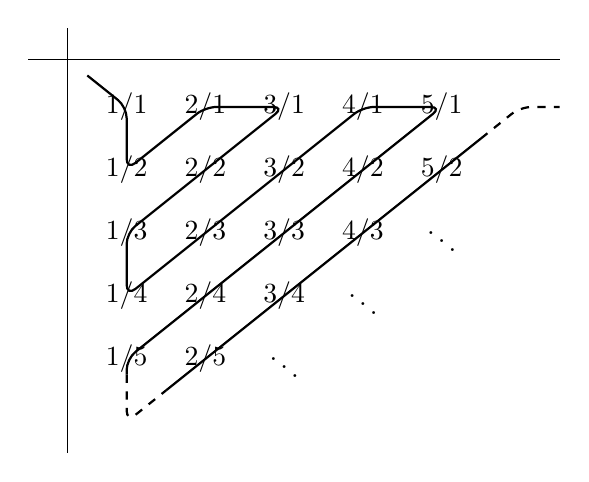
\begin{tikzpicture}[yscale=-0.8]

%\node at (0,0) {$0$};
\foreach \x in {1,2,3,4,5} \foreach \y in {1,2} { \node at (\x,\y) {$\x/\y$}; }
\foreach \x in {1,2,3,4} { \node at (\x,3) {$\x/3$}; }
\foreach \x in {1,2,3} { \node at (\x,4) {$\x/4$}; }
\foreach \x in {1,2} { \node at (\x,5) {$\x/5$}; }
%\node at (6,1.5) {$\cdots$};
\node at (5,3) {$\ddots$};
\node at (3,5) {$\ddots$};
\node at (4,4) {$\ddots$};
%\node at (1.5,6) {$\vdots$};
\draw (-0.25,0.25) -- (6.5,0.25);
\draw (0.25,-0.25) -- (0.25,6.5);
\draw[thick,rounded corners=4pt] (0.5,0.5) -- (1,1) -- (1,2) -- (2,1) -- (3,1) -- (2,2) -- (1,3)
  -- (1,4) -- (2,3) -- (3,2) -- (4,1) -- (5,1) -- (4,2) -- (3,3) -- (2,4) -- (1,5) -- (1,5.25);
\draw[thick,rounded corners=4pt,dashed] (1,5.25) -- (1,6) -- (1.5,5.5);
\draw[thick,rounded corners=4pt] (1.5,5.5) -- (2,5) -- (3,4) -- (4,3) -- (5,2) -- (5.5,1.5);
\draw[thick,rounded corners=4pt,dashed] (5.5,1.5) -- (6,1) -- (6.5,1);

\end{tikzpicture}
